\newpage
\pagenumbering{Roman}
\setcounter{page}{8}    %manuell römische Seitenzahl einstellen! 

\begin{appendix}
\clearpage{}

%Erste Seite eines pdf-Anhangs mit Überschrift:

\includepdf[scale=0.9,pages=1,pagecommand={\chapter{Ein PDF Anhang} }, offset=0 0.5cm]{test3}
%Weitere Seiten ohne zusätzliche Überschrift:

\includepdf[scale=0.9,pages=2-3,pagecommand={}, offset=0 0.5cm]{test3} %Pagecommand, dafür dass die Seitenzahl nicht verschwindet



%Graphiken einfügen
\chapter{Ein Tabellenanhang}
\begin{figure}[ht]
	\centering
  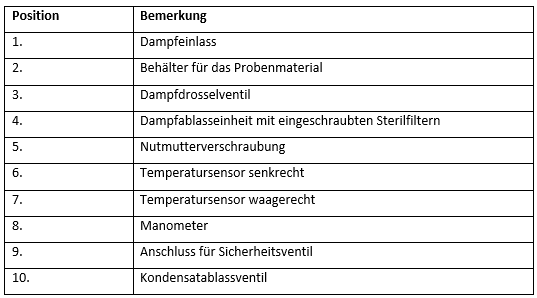
\includegraphics[width=\textwidth] {Anhang/tabelle1.png}
	%\caption{um 30 Grad gedreht}
	%\label{fig1}
\end{figure}

\end{appendix}
